\documentclass[11pt]{article}

\usepackage{amsmath}
\usepackage{amssymb}
\usepackage{graphicx}
\usepackage{caption}
\usepackage{subcaption}

\topmargin -.5in
\textheight 9in
\oddsidemargin -.25in
\evensidemargin -.25in
\textwidth 7in

\newcommand{\code}[1]{\texttt{#1}}

\begin{document}

\author{Gu, Qiao}
\title{16-720B Homework 2 Write-up}
\maketitle

\medskip

\subsection*{Q1.2}

Please see Figure.~\ref{fig:q1.2} for the DoG Pyramid of \code{model\_chickenbroth.jpg}.

\begin{figure}[h!]
    \centering
    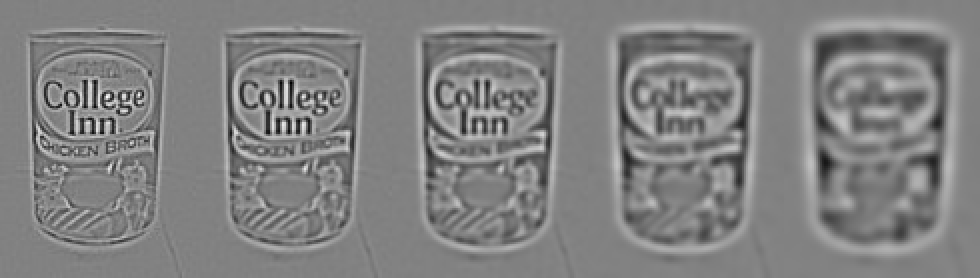
\includegraphics[width=.8\linewidth]{../results/q1_2.png}
    \caption{The DoG Pyramid of \code{model\_chickenbroth.jpg}}
    \label{fig:q1.2}
\end{figure}

\newpage

\subsection*{Q1.5}

Please see Figure.~\ref{fig:q1.5} for the detected keypoints of \code{model\_chickenbroth.jpg}.

\begin{figure}[h!]
    \centering
    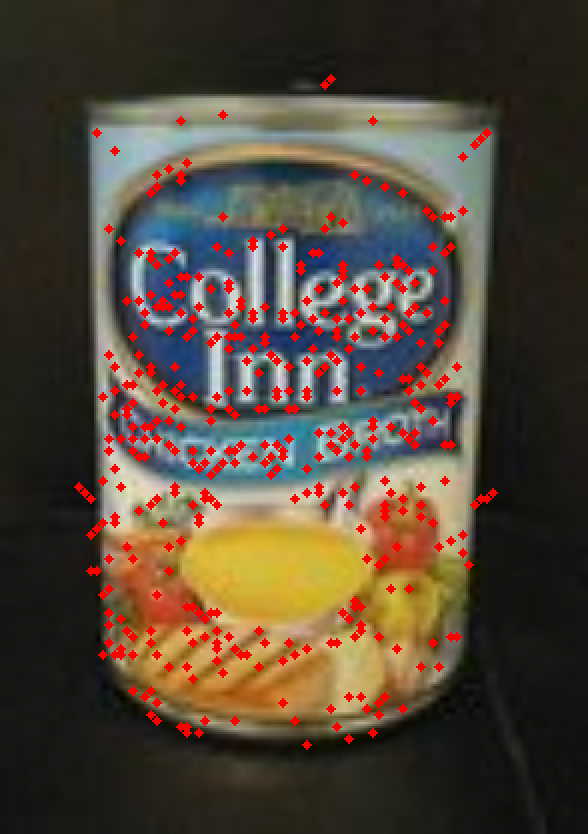
\includegraphics[width=.4\linewidth]{../results/q1_5.png}
    \caption{The detected keypoints on image \code{model\_chickenbroth.jpg}}
    \label{fig:q1.5}
\end{figure}

\newpage

\subsection*{Q2.4}

Please see Figure~\ref{fig:q2.4} for the matching results. From the results, we can see that if the object is rotated, the matching performance will be much worse than those with little or no rotation (compare Figure.~\ref{fig:q2.4} (d)(g) with Figure.~\ref{fig:q2.4} (c)(f)). I suspect this is because the BRIEF descriptor does not encode the patch into a rotation-invariant space and thus have poor ability to match rotated patches.

\begin{figure}[h!] \label{fig:q2.4}
    \begin{subfigure}{.49\textwidth}
      \centering
      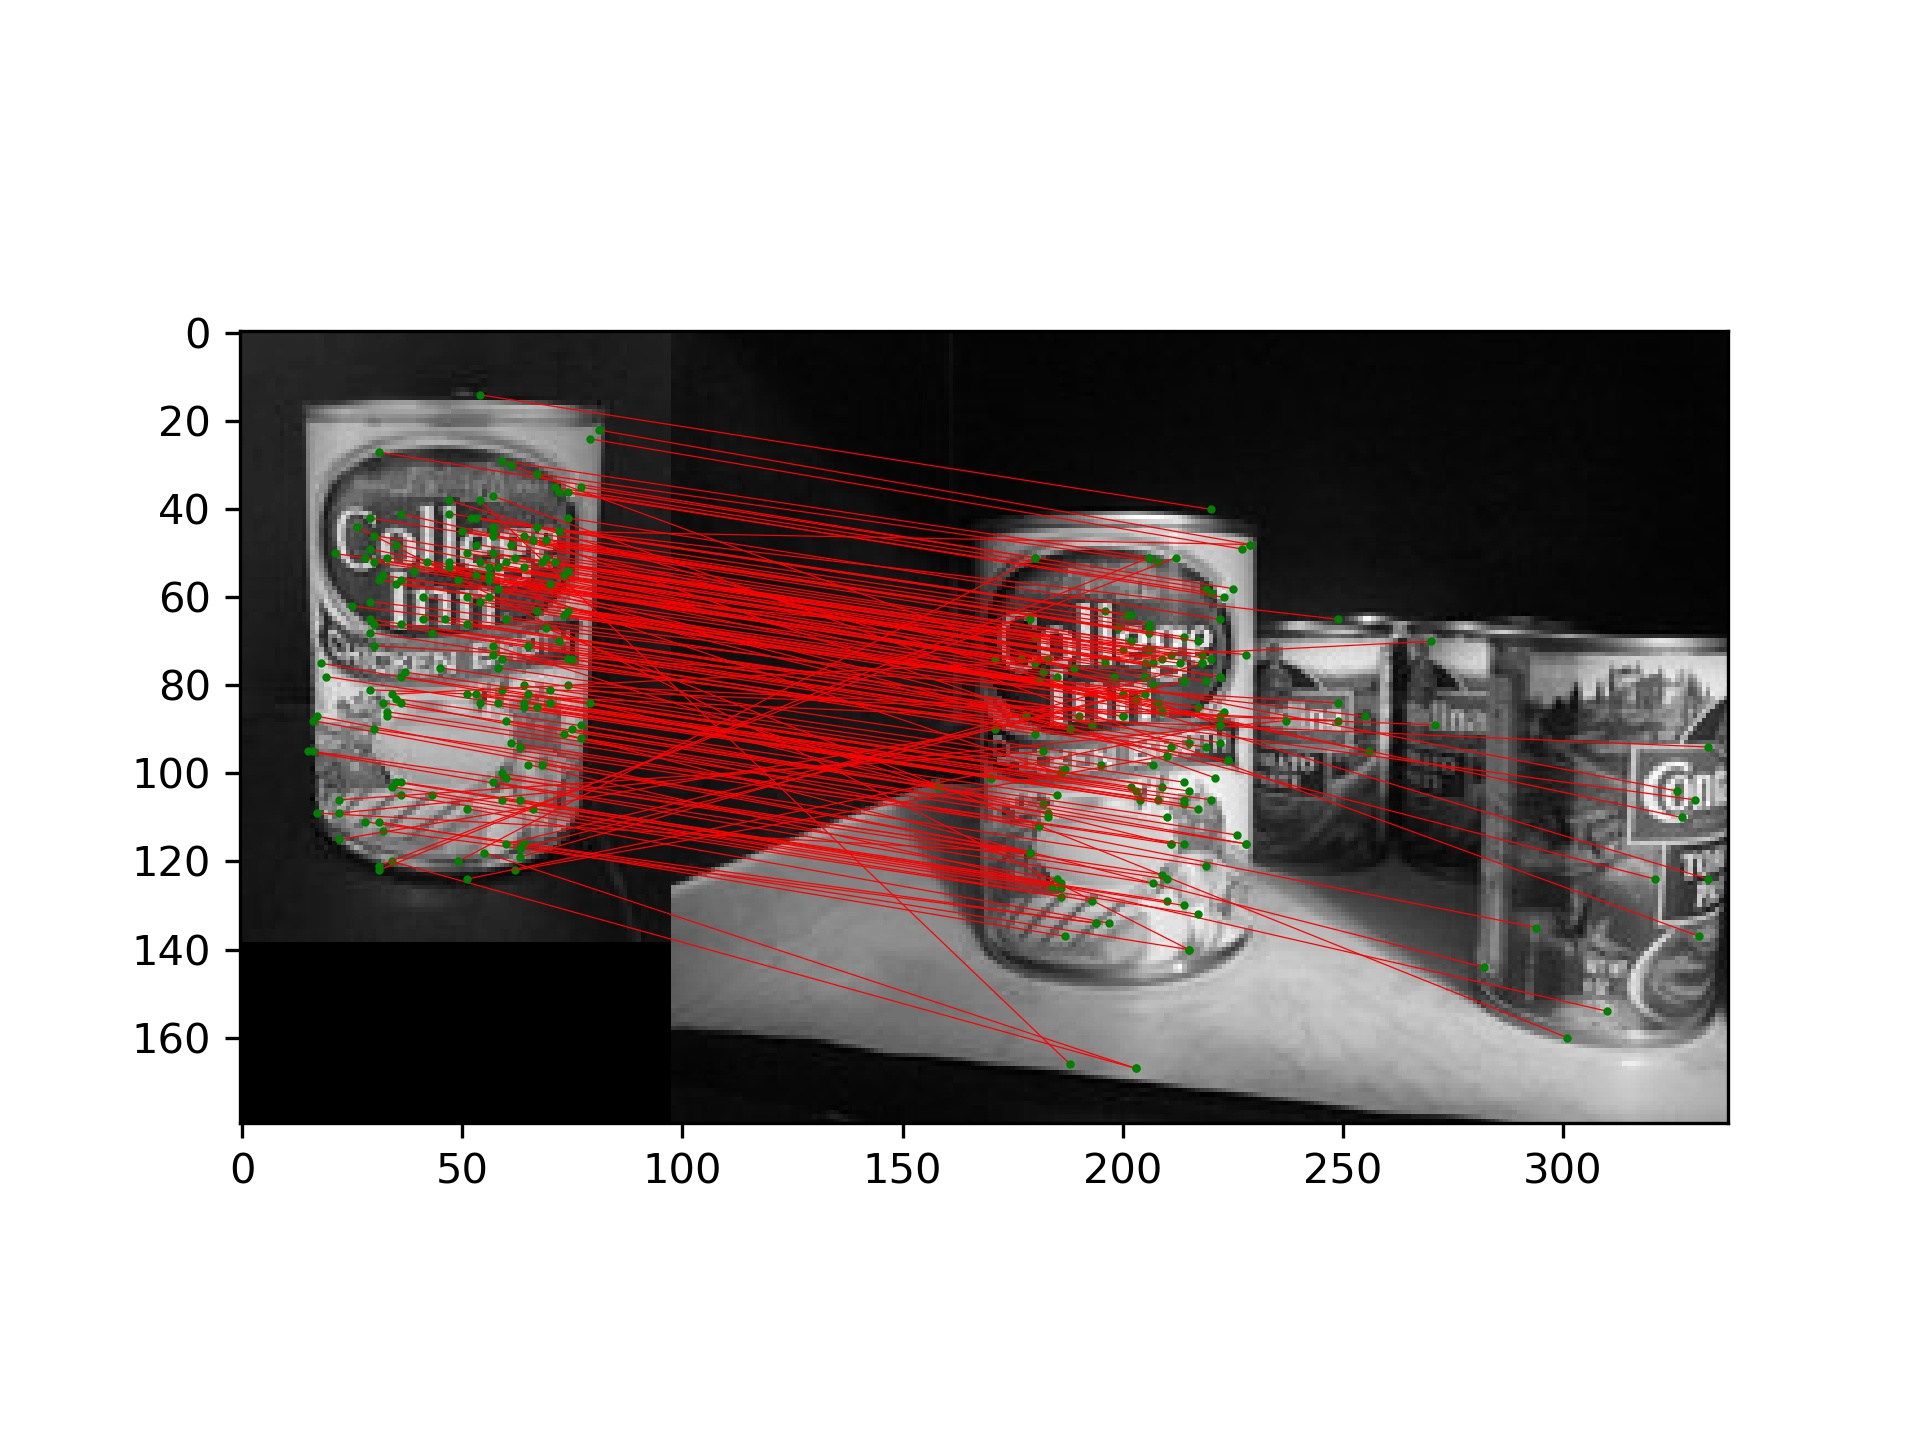
\includegraphics[width=.8\linewidth]{../results/chickenbroth_01_match.jpg}
      \caption{match of two of the \code{chickenbroth} images.}
    \end{subfigure}
    \begin{subfigure}{.49\textwidth}
      \centering
      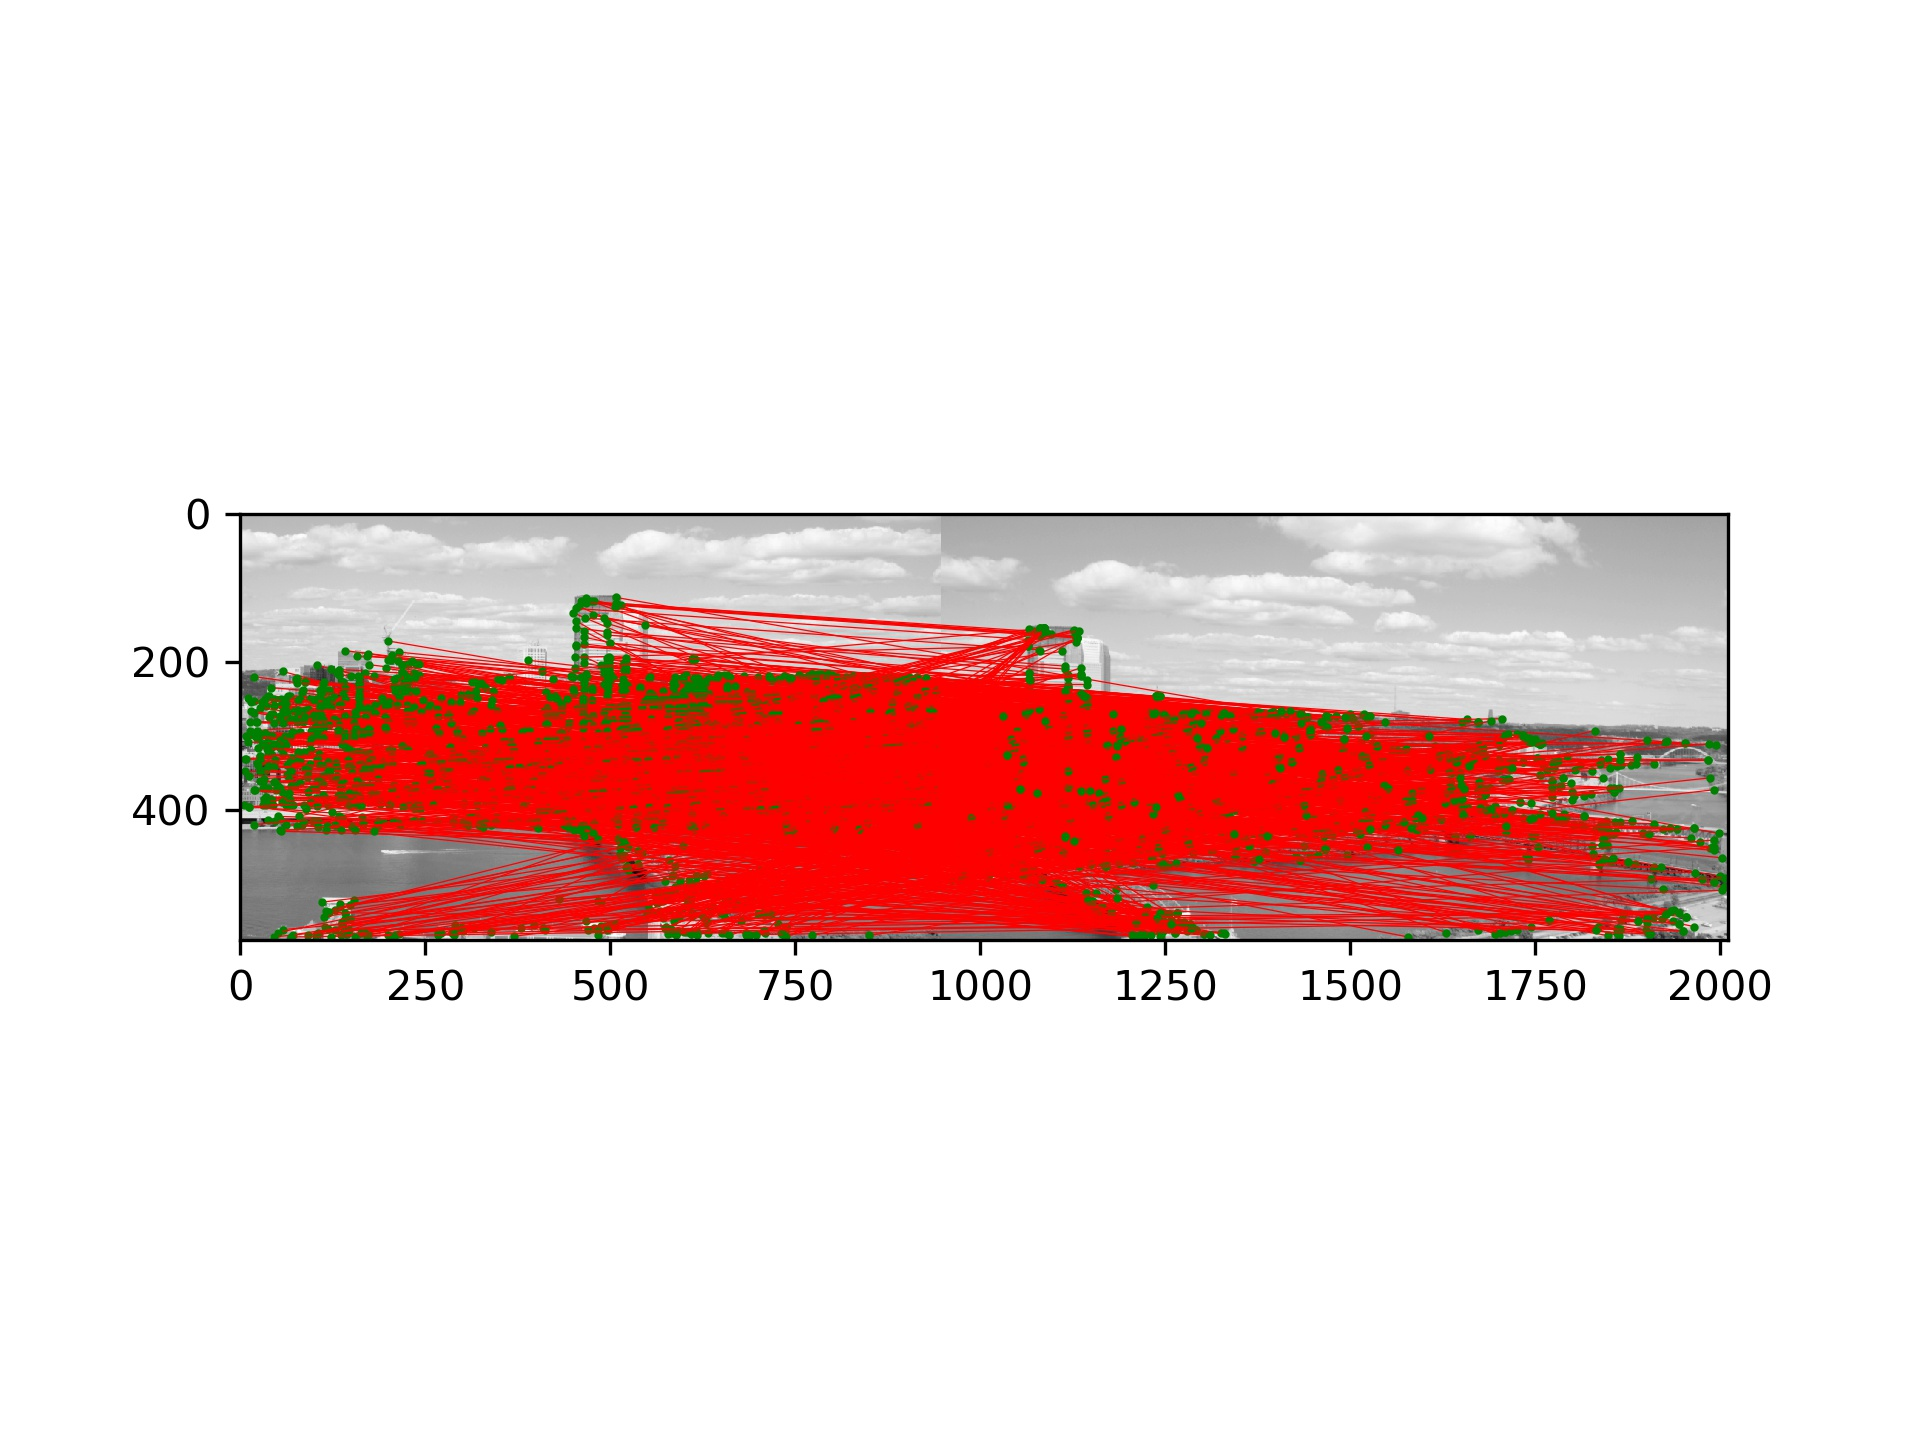
\includegraphics[width=.8\linewidth]{../results/incline_match.jpg}
      \caption{match of the \code{incline} images. }
    \end{subfigure}
    \begin{subfigure}{.327\textwidth}
      \centering
      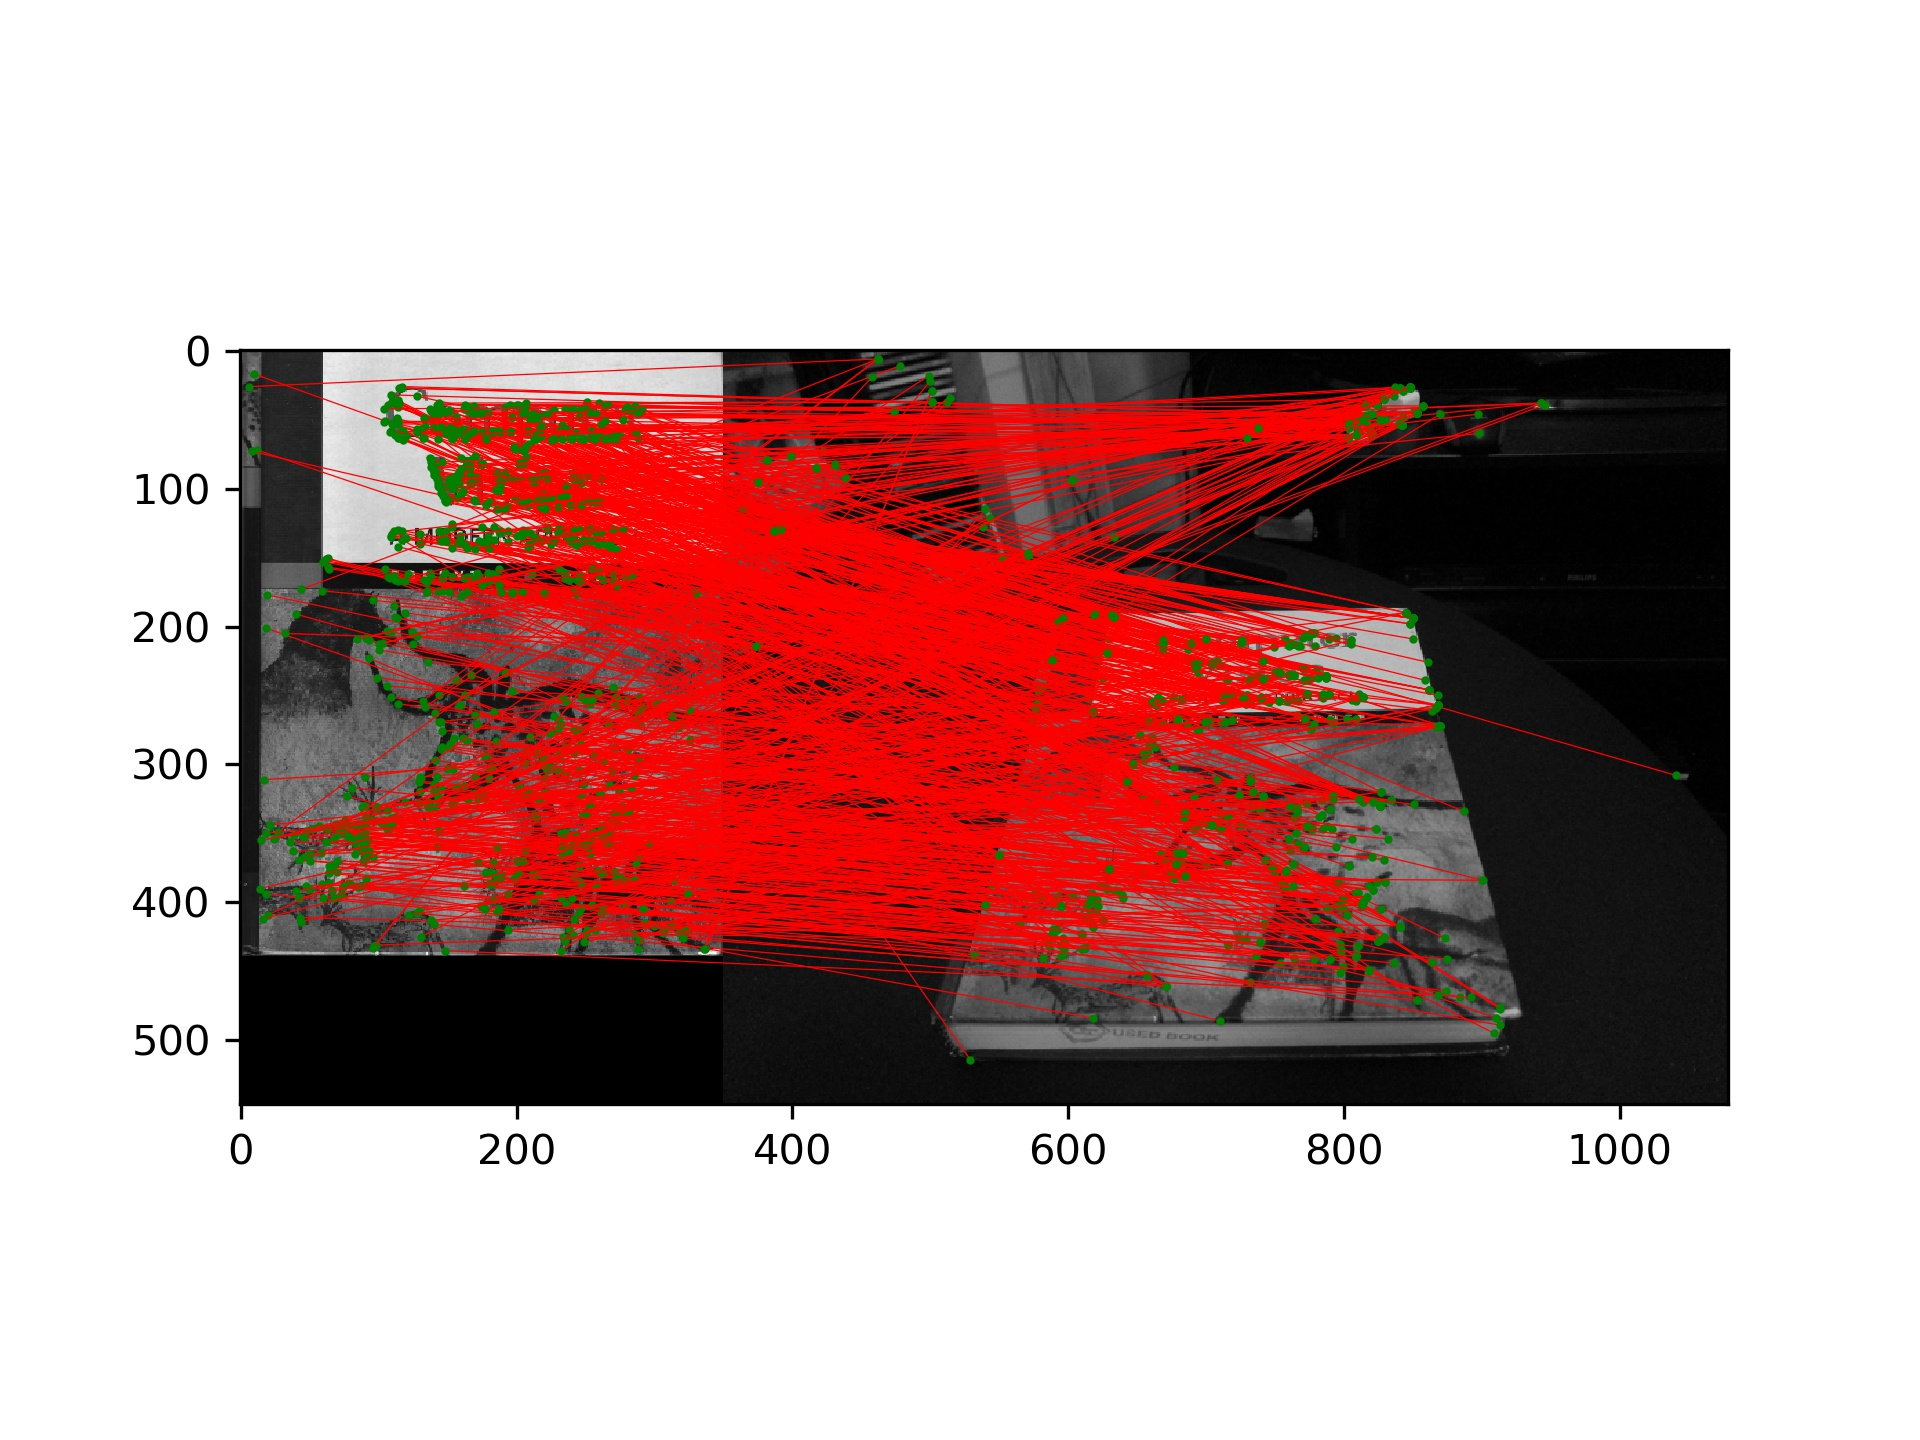
\includegraphics[width=.8\linewidth]{../results/pf_desk_match.jpg}
      \caption{match of \code{pf\_scan\_scaled.jpg} against \code{pf\_desk.jpg}.}
    \end{subfigure}
    \begin{subfigure}{.327\textwidth}
      \centering
      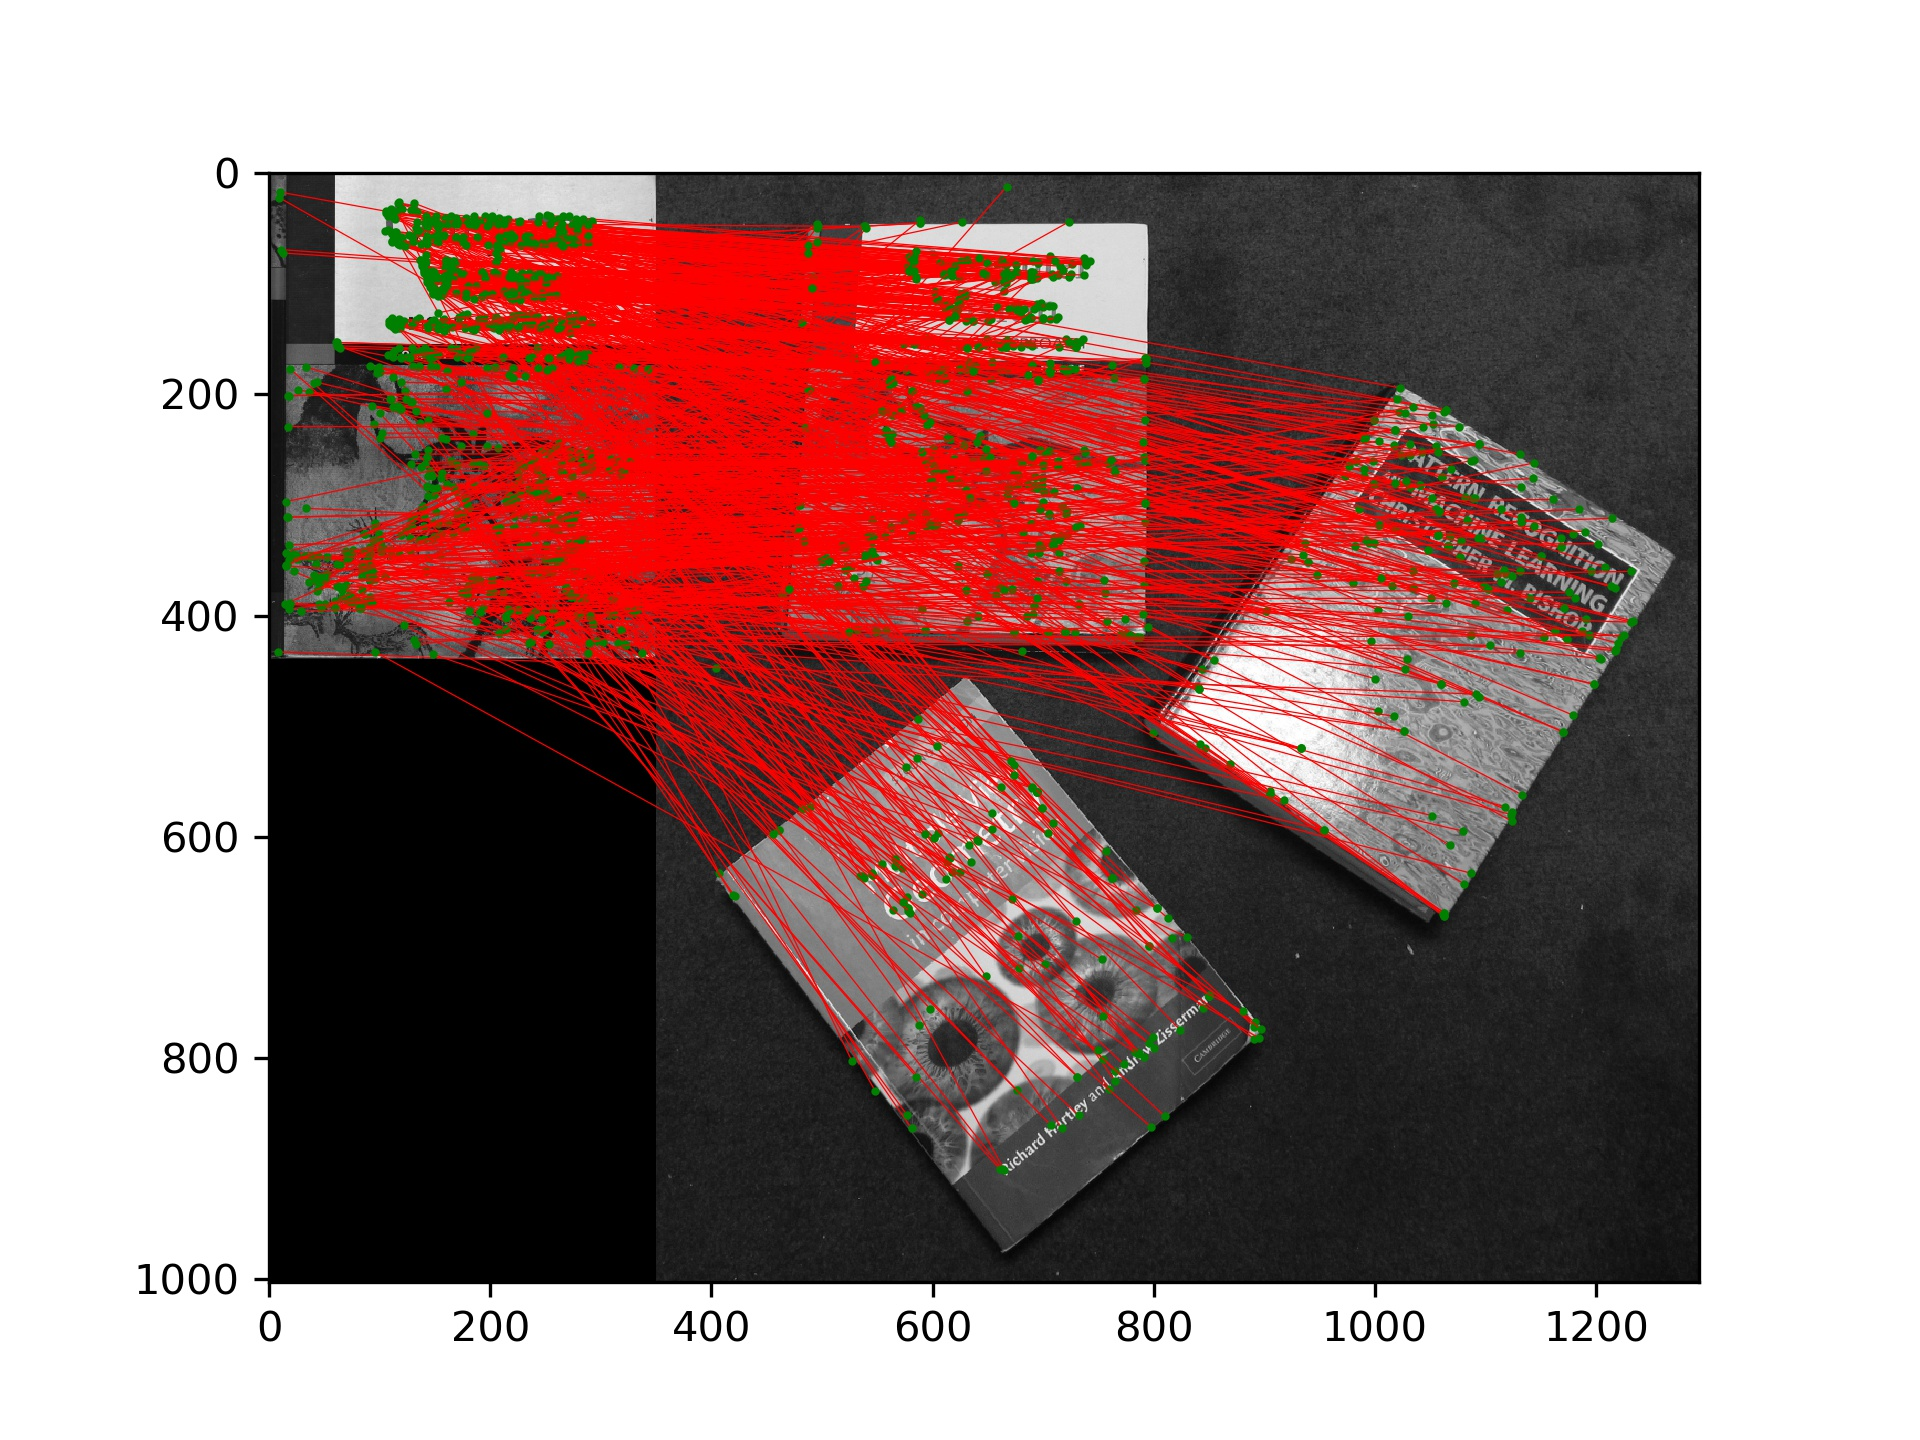
\includegraphics[width=.8\linewidth]{../results/pf_floor_match.jpg}
      \caption{match of \code{pf\_scan\_scaled.jpg} against \code{pf\_floor.jpg}.}
    \end{subfigure}
    \begin{subfigure}{.327\textwidth}
      \centering
      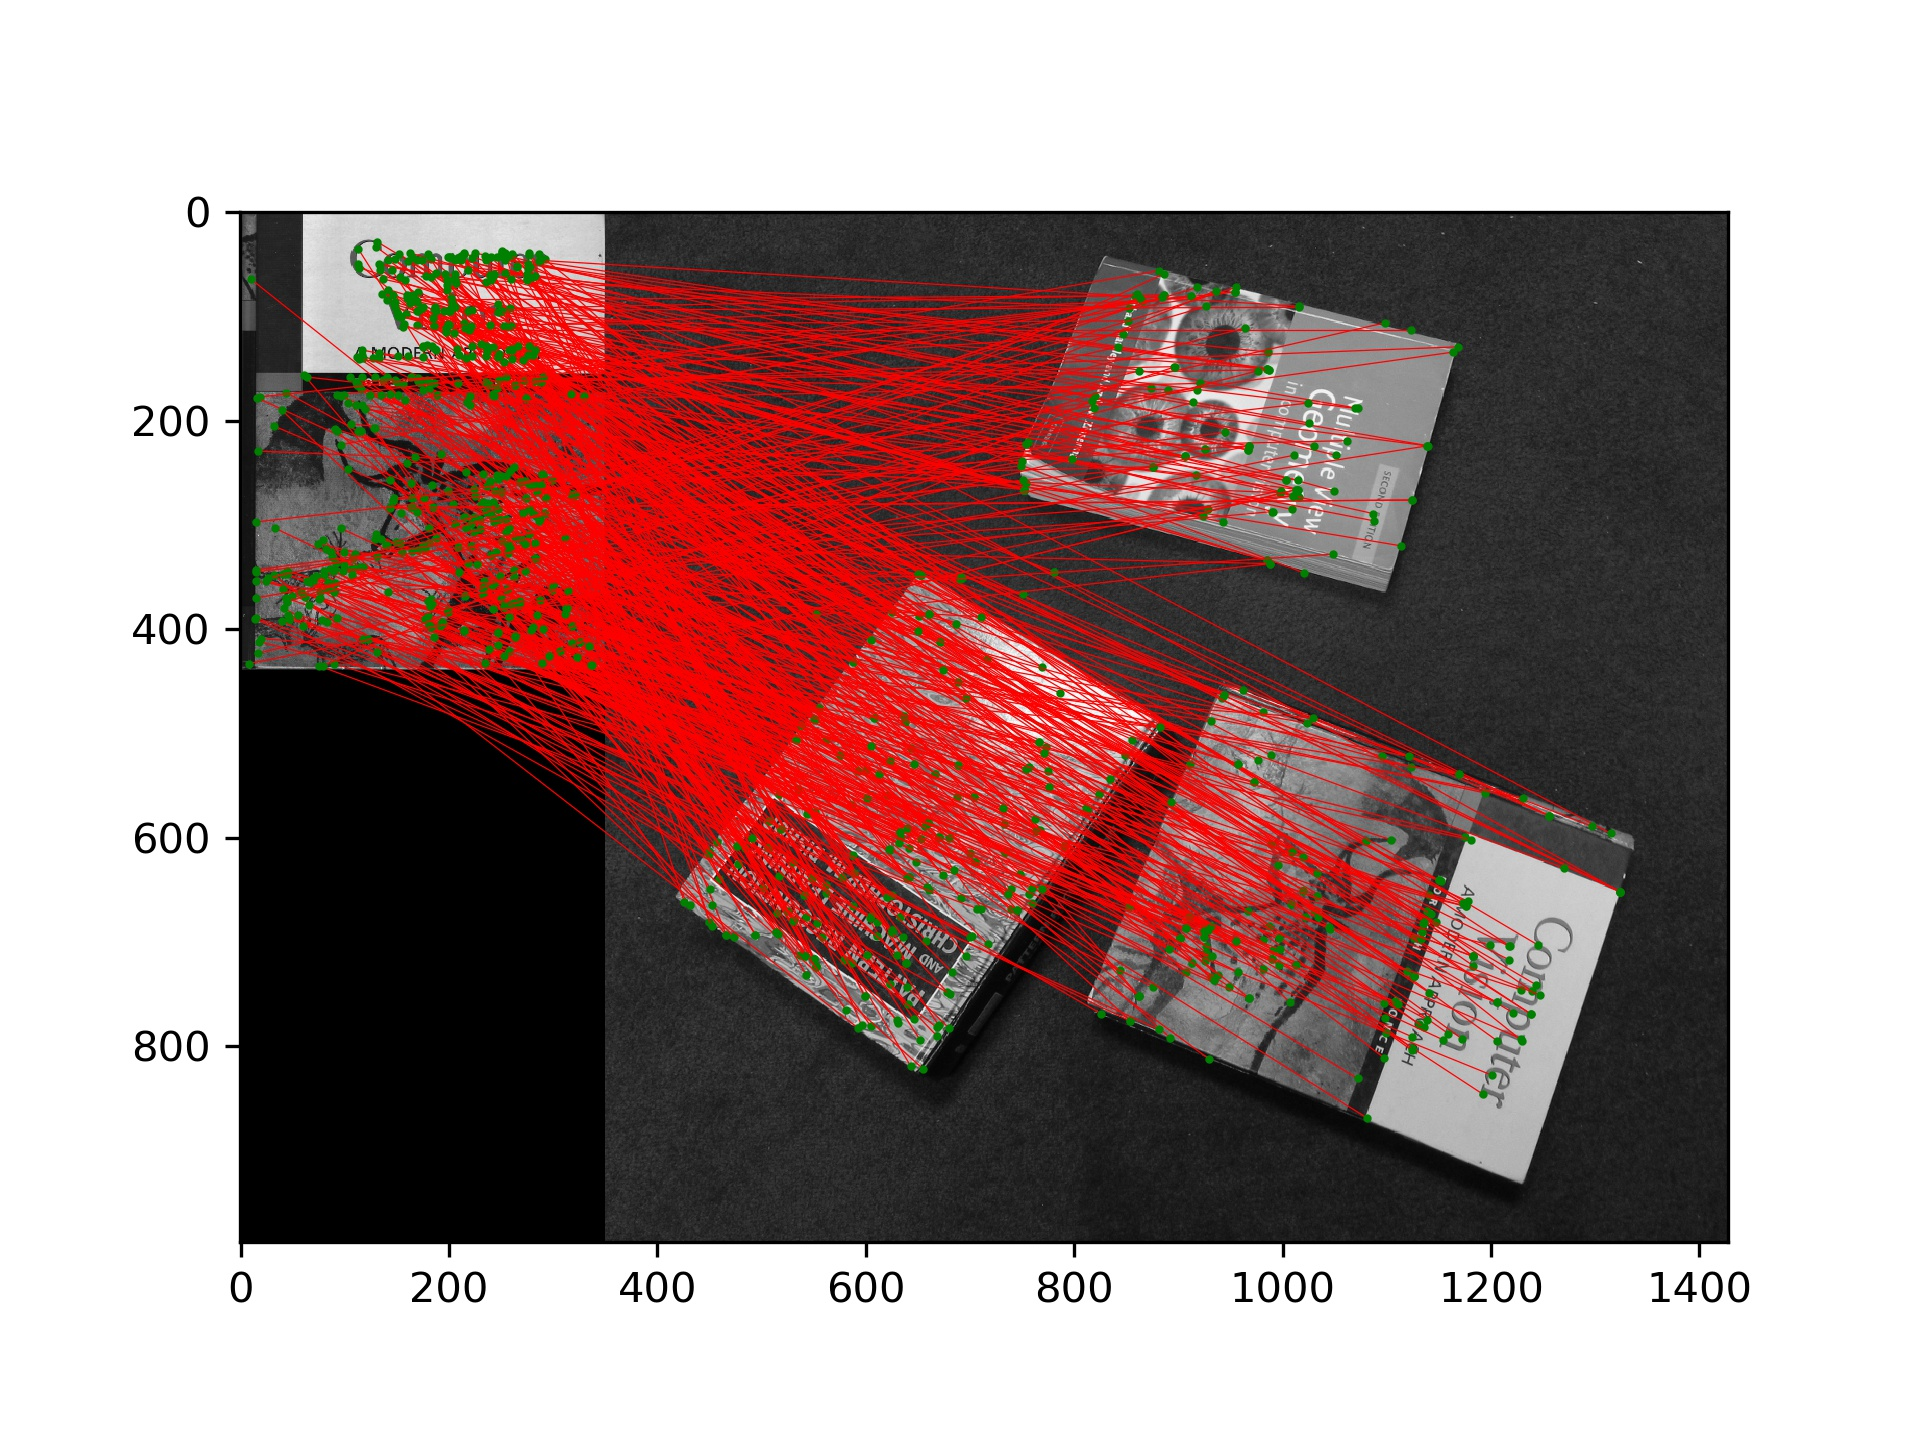
\includegraphics[width=.8\linewidth]{../results/pf_floor_rot_match.jpg}
      \caption{match of \code{pf\_scan\_scaled.jpg} against \code{pf\_floor\_rot.jpg}.}
    \end{subfigure}
    \begin{subfigure}{.327\textwidth}
      \centering
      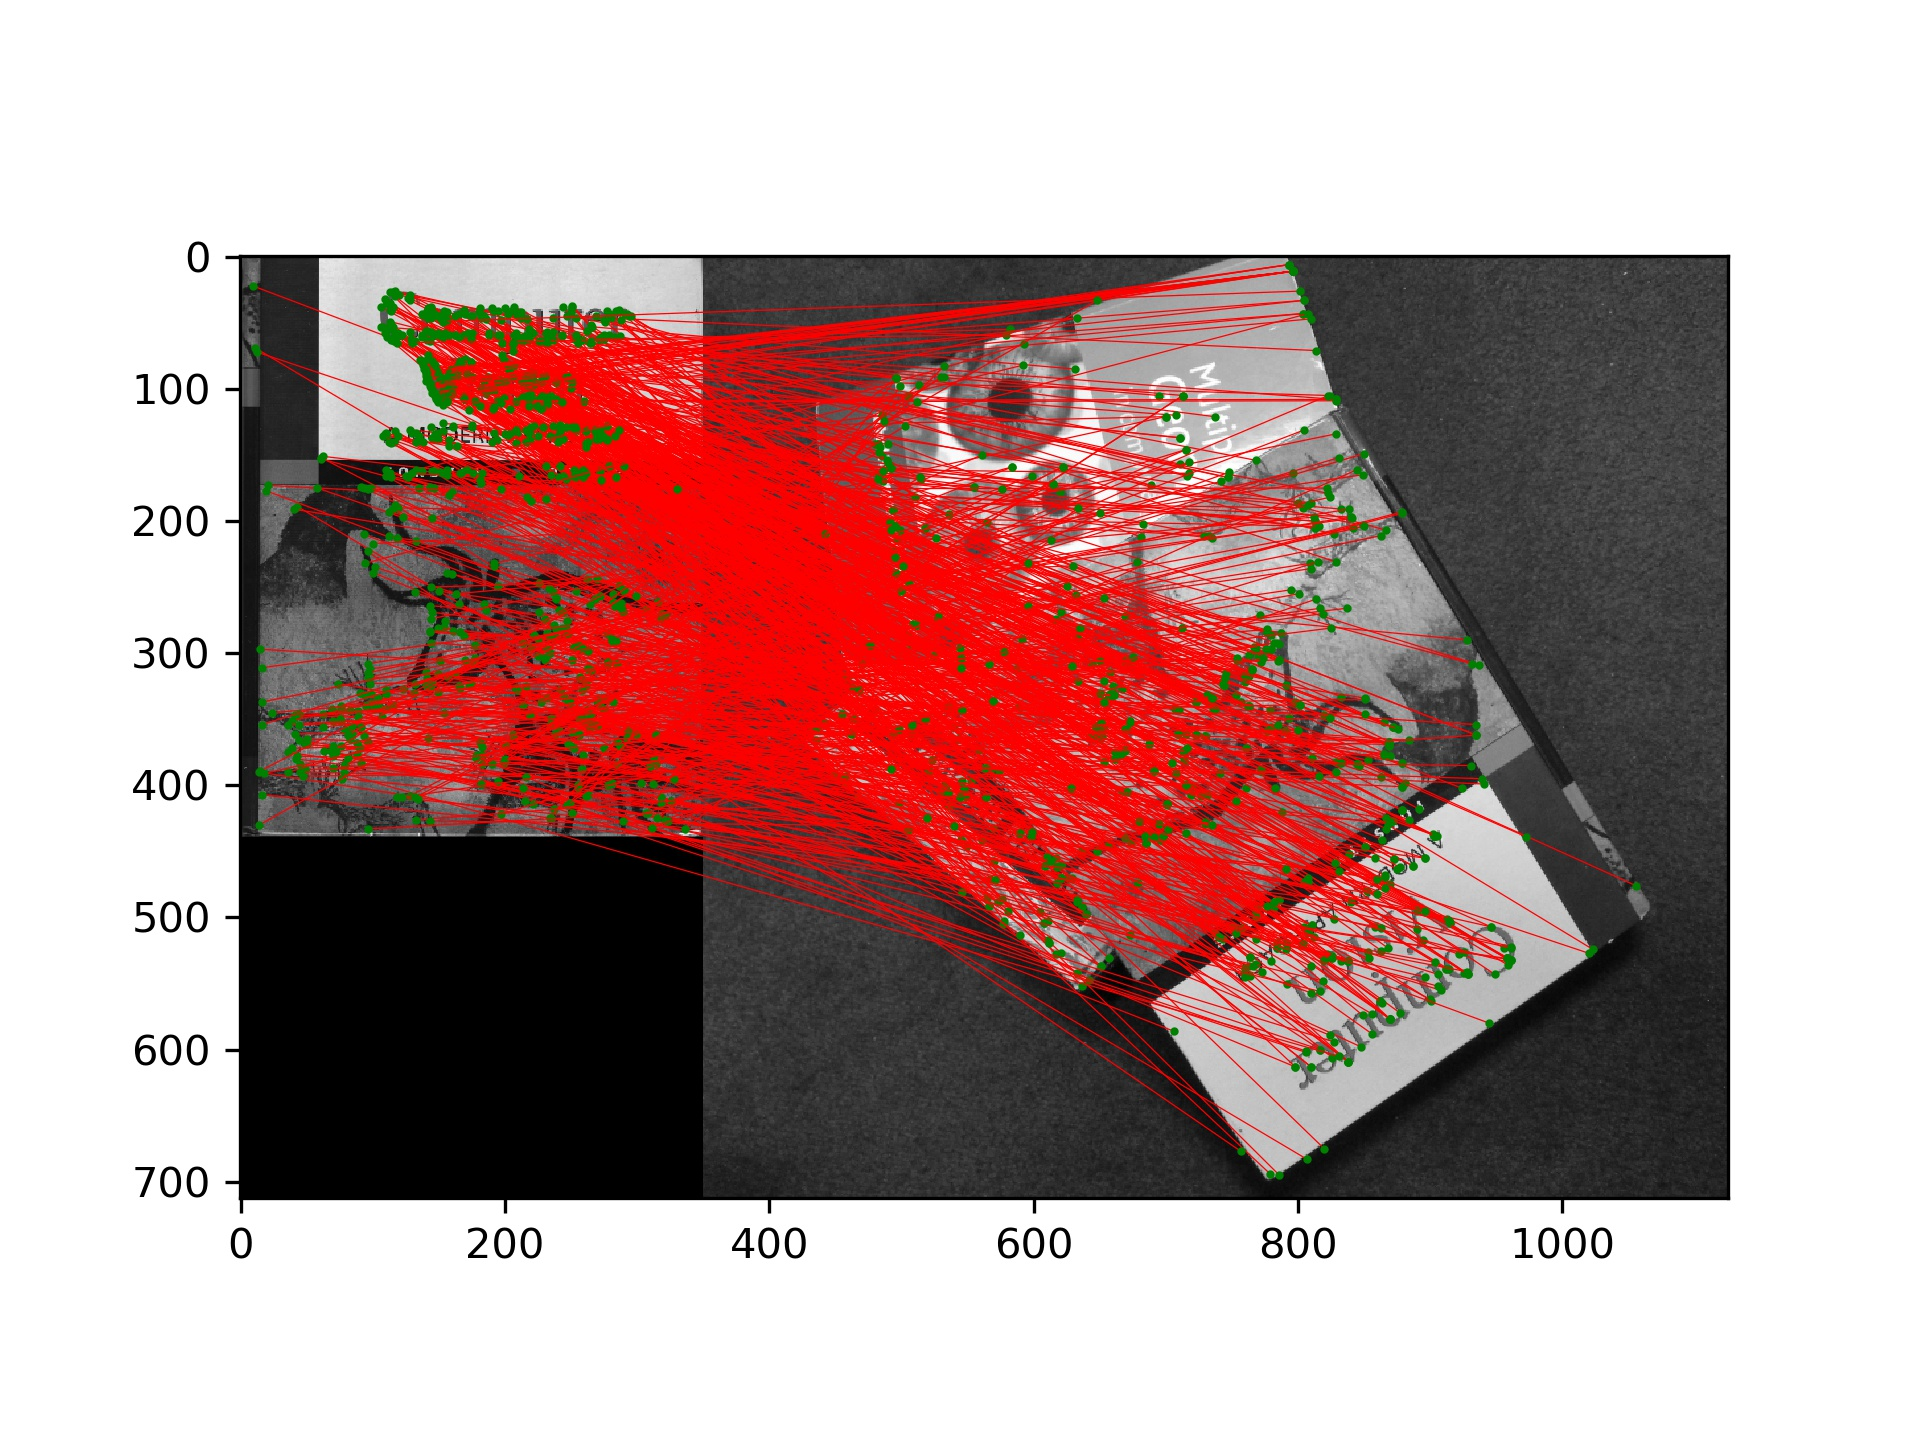
\includegraphics[width=.8\linewidth]{../results/pf_pile_match.jpg}
      \caption{match of \code{pf\_scan\_scaled.jpg} against \code{pf\_pile.jpg}.}
    \end{subfigure}
    \begin{subfigure}{.327\textwidth}
      \centering
      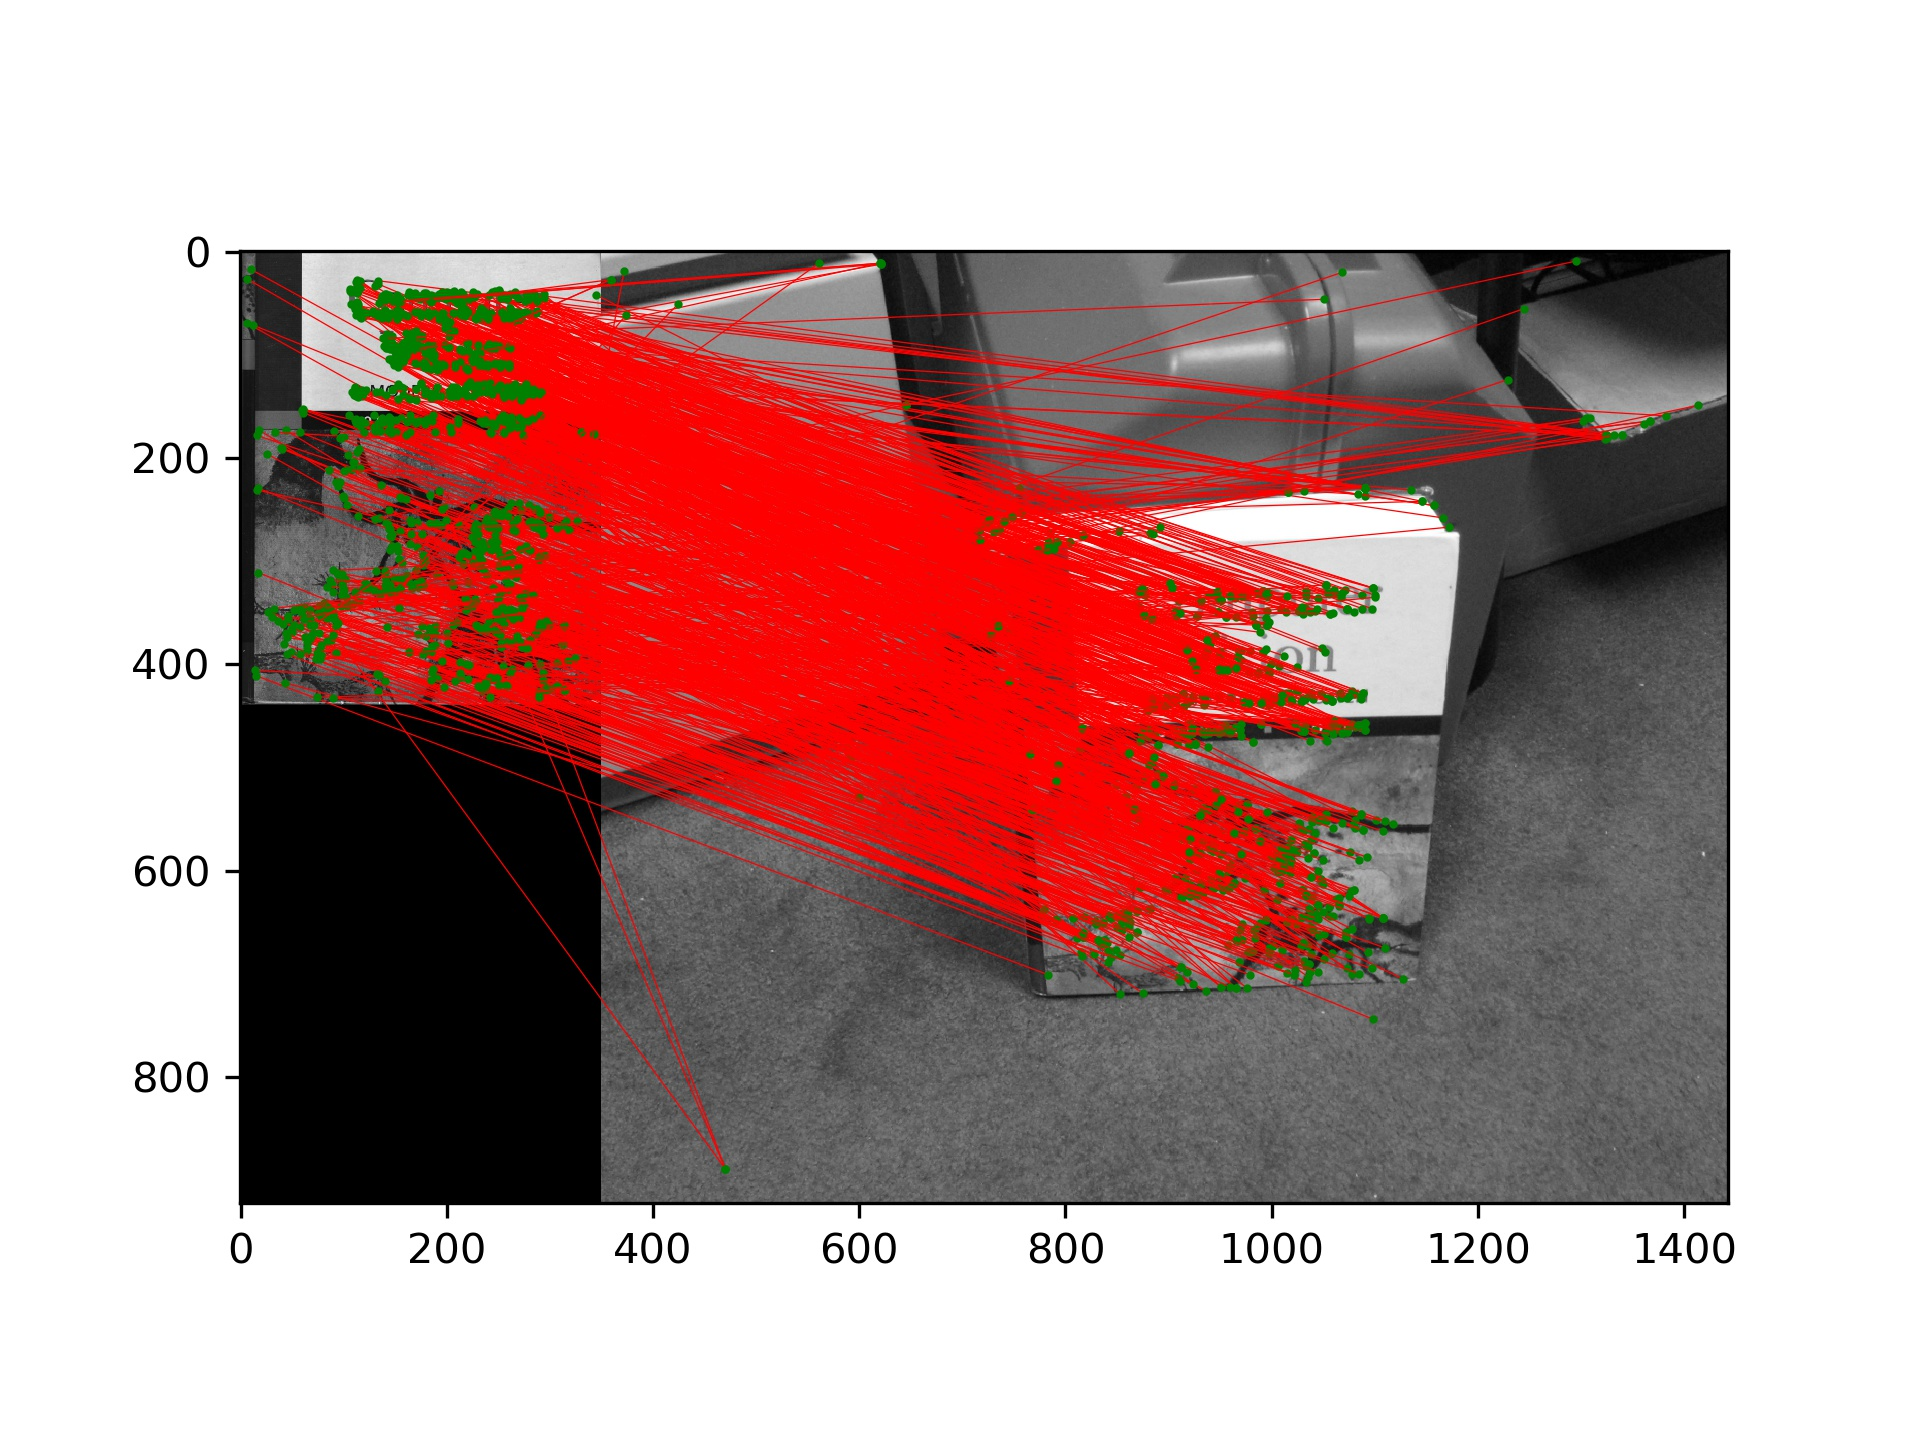
\includegraphics[width=.8\linewidth]{../results/pf_stand_match.jpg}
      \caption{match of \code{pf\_scan\_scaled.jpg} against \code{pf\_stand.jpg}.}
    \end{subfigure}
    \caption{Results of Feature Match. }
    \label{fig:q2.4}
\end{figure}

\newpage

\subsection*{Q2.5}

Please see Figure~\ref{fig:q2.5} for the matching results. As we can see, the number of matches reaches its maximum when there is no rotation between two images, and drops quickly when the rotation angle starts to increase. This is probably because the BRIEF descriptor we Implement only treats each keypoint patch as a rectangle grid, and thus when the rectangle is rotated, the whole grid structure can be messed up. Therefore the number of matches drops quickly as with rotation.

\begin{figure}[h!]
    \centering
    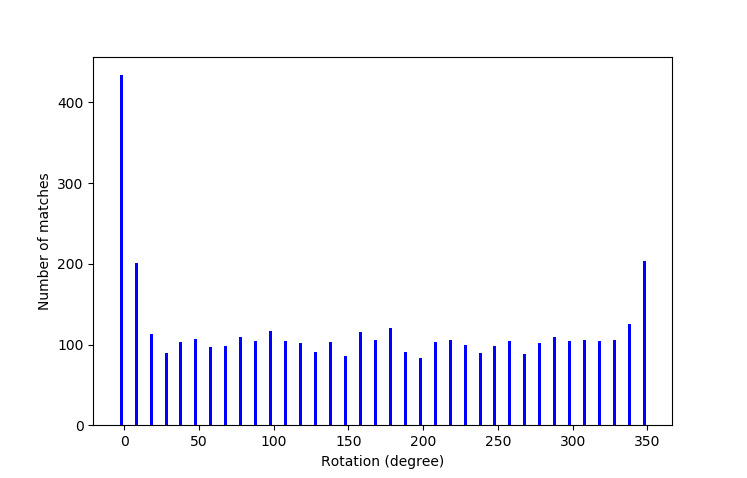
\includegraphics[width=.8\linewidth]{../results/q2_5.png}
    \caption{The rotation angle vs the number of correct matches}
    \label{fig:q2.5}
\end{figure}

\newpage

\subsection*{Q3.1}

\subsubsection*{Q3.1.1}

\newcommand{\vecxn}{\tilde{\mathbf{x}_n}}
\newcommand{\vecun}{\tilde{\mathbf{u}_n}}

From the given equation $\lambda_n \vecxn = \mathbf{H} \vecun$, we can get

\begin{equation}
    \lambda_n
    \begin{bmatrix}
        x_{n} \\ y_{n} \\ 1
    \end{bmatrix}
    =
    \begin{bmatrix}
        H_{11} & H_{12} & H_{13} \\
        H_{21} & H_{22} & H_{23} \\
        H_{31} & H_{32} & H_{33}
    \end{bmatrix}
    \begin{bmatrix}
        u_{n} \\ v_{n} \\ 1
    \end{bmatrix}.
\end{equation}

And change it to equations:

\begin{align}
    \lambda_n x_{n} = H_{11} u_{n} + H_{12} v_{n} + H_{13} \\
    \lambda_n y_{n} = H_{21} u_{n} + H_{22} v_{n} + H_{23} \\
    \lambda_n = H_{31} u_{n} + H_{32} v_{n} + H_{33} .
\end{align}

Then elinimate $\lambda_n$:

\begin{align}
    H_{31} u_{n} x_{n} + H_{32} v_{n} x_{n} + H_{33} x_{n} = H_{11} u_{n} + H_{12} v_{n} + H_{13} \\
    H_{31} u_{n} y_{n} + H_{32} v_{n} y_{n} + H_{33} y_{n} = H_{21} u_{n} + H_{22} v_{n} + H_{23},
\end{align}

which is equivalent to:

\begin{equation}
    \begin{bmatrix}
        u_{n} & v_{n} & 1 & 0 & 0 & 0 & -u_{n} x_{n} & -v_{n} x_{n} & -x_{n} \\
        0 & 0 & 0 & u_{n} & v_{n} & 1 & -u_{n} y_{n} & -v_{n} y_{n} & -y_{n} \\
    \end{bmatrix}
    \begin{bmatrix}
        H_{11} \\ H_{12} \\ H_{13} \\
        H_{21} \\ H_{22} \\ H_{23} \\
        H_{31} \\ H_{32} \\ H_{33}
    \end{bmatrix}
    = \mathbf{0}
\end{equation}

Repeat the equation above for $n=1...N$, then we can get:

\begin{equation}
    \begin{bmatrix}
        u_{1} & v_{1} & 1 & 0 & 0 & 0 & -u_{1} x_{1} & -v_{1} x_{1} & -x_{1} \\
        0 & 0 & 0 & u_{1} & v_{1} & 1 & -u_{1} y_{1} & -v_{1} y_{1} & -y_{1} \\
        &&&&&\cdots &&& \\
        u_{N} & v_{N} & 1 & 0 & 0 & 0 & -u_{N} x_{N} & -v_{N} x_{N} & -x_{N} \\
        0 & 0 & 0 & u_{N} & v_{N} & 1 & -u_{N} y_{N} & -v_{N} y_{N} & -y_{N} \\
    \end{bmatrix}
    \begin{bmatrix}
        H_{11} \\ H_{12} \\ H_{13} \\
        H_{21} \\ H_{22} \\ H_{23} \\
        H_{31} \\ H_{32} \\ H_{33}
    \end{bmatrix}
    = \mathbf{0}
\end{equation}

The $2N\times 2$ matrix on the left hand side is the $\mathbf{A}$ required, and the other one is $\mathbf{h}$

\subsubsection*{Q3.1.2}

There are 9 elements in $\mathbf{h}$,

\subsubsection*{Q3.1.3}

Since we can add a constraint that $\mathbf{h} = 1$. Therefore there are 8 free elements left in $\mathbf{h}$, and thus 8 degress of freedom in $\mathbf{H}$.

We only need 4 correspondence to solve this system, since each point correspondence provide 2 equations that solve 2 degree of freedom.

\subsubsection*{Q3.1.4}

\newcommand{\norm}[1]{\left\lVert#1\right\rVert}

The problem can be formulated as

\begin{equation}
    \mathbf{Ah} = \mathbf{0} \quad
    \textrm{s.t.} \; \norm{\mathbf{h}}_2 = 1 .
\end{equation}

When we have more than 4 correspondence, a accurate solution cannot be found and thus the problem becomes a least square problem as follows:

\begin{align}
    & \arg\min_{\mathbf{h}} \norm{\mathbf{Ah}}^2_2
    \quad \textrm{s.t.} \; \mathbf{h}^T \mathbf{h} = 1
    \\ \Leftrightarrow
    & \arg\min_{\mathbf{h}}
    \frac{\mathbf{h}^T\mathbf{A}^T\mathbf{A}\mathbf{h}}{\mathbf{h}^T\mathbf{h}}
    \quad \textrm{s.t.} \; \mathbf{h}^T \mathbf{h} = 1
\end{align}

The expression on the L.H.S. in the above equation is the Rayleigh quotient of the matrix $A^T A$, and its minimum is the minimum eigenvalue $\lambda_{min}$ of $A^T A$. Therefore, if we can find the singular value decomposition $\mathbf{A} = \mathbf{U\Sigma V}^T$, the solution $\mathbf{h}$ will be the right singular vector $v_9$ corresponding to the minimum singular value $\sigma_{min}=\sigma_9$ of $\mathbf{A}$. (Note that $\mathbf{A}\in \mathbb{R}^{2N\times 9}$ and $\mathbf{A}^T\mathbf{A}\in \mathbb{R}^{9\times 9}$)

\newpage

\subsection*{Q6.1}



\end{document}
